\documentclass[12pt,a4paper]{report}
\usepackage[utf8]{inputenc}
\usepackage[explicit]{titlesec}
\usepackage[dvipsnames]{xcolor}
\usepackage{amsmath}
\usepackage{amsfonts}
\usepackage{url}
\usepackage{amssymb}
\usepackage{makeidx}
\usepackage{graphicx}
\usepackage{tikz}
\usepackage[many]{tcolorbox}
\usepackage{standalone}
\usepackage{animate}
\tcbuselibrary{listings}
\usepackage{tabularx}
\usepackage{colortbl}
\usepackage{multicol}
\usepackage{makecell}
\usepackage{adjustbox}
\usepackage{subfig}
\usepackage{lipsum}
\usepackage{float} % Added for figure positioning

\usepackage{framed}
\usepackage{lastpage}

\usepackage{fancyhdr}
% Combined TikZ libraries from template and draft
\usetikzlibrary{calc,arrows.meta,backgrounds,shapes.geometric,positioning}

\newcommand{\msymbol}[1]{\ifmmode #1 \else $#1$\fi}

\newcommand{\daemathvariable}[1]{{\normalsize \color[RGB]{100,149,237}#1}}
\newcommand{\daemathvalue}[1]{{\normalsize \color[RGB]{153,153,255}#1}}
\newcommand{\daemath}[1]{{\large \color[RGB]{0,0,0}#1}}
\newcommand{\daered}[1]{{\normalsize \color[RGB]{234,0,33}#1}}
\newcommand{\daegreen}[1]{{\normalsize \color[RGB]{0,255,65}#1}}
\newcommand{\mmathvariable}[1]{{\begingroup  \color[RGB]{100,149,237}#1 \endgroup} }
\newcommand{\mmathvalue}[1]{{\begingroup  \color[RGB]{153,153,255}#1 \endgroup} }
\newcommand{\mmath}[1]{{\begingroup  \color[RGB]{0,0,0}#1 \endgroup} }
\newcommand{\mred}[1]{{\begingroup  \color[RGB]{234,0,33}#1 \endgroup} }
\newcommand{\mgreen}[1]{{\begingroup  \color[RGB]{0,255,65}#1 \endgroup} }
\definecolor{backgroundStroke}{RGB}{0,0,0}
\definecolor{backgroundFill}{RGB}{255,255,255}
\definecolor{backgroundText}{RGB}{0,0,0}
\definecolor{bgChapter}{RGB}{91,155,213}
\definecolor{bgSection}{RGB}{222,234,246}
\definecolor{fontSubsection}{RGB}{53,124,177}
\colorlet{shadecolor}{bgChapter}

\renewcommand{\contentsname}{Contents}
\newcommand{\pbreak}{\vskip 0.5cm}
\renewcommand{\thesection}{\arabic{section}}

\newcommand{\daechapter}[1]{
  \chapter*{#1} % Create an unnumbered chapter
  \addcontentsline{toc}{chapter}{#1} % Add the chapter to the ToC
}

\newcommand{\daesection}[1]{
  \section*{#1} % Create an unnumbered chapter
  \addcontentsline{toc}{chapter}{#1} % Add the chapter to the ToC
}

\newtcolorbox{ybox}{
  colback=yellow,
  colframe=yellow,
  boxrule=0pt,
  arc=0pt,
  outer arc=0pt,
  boxsep=0pt,
  left=1pt,
  right=1pt,
  top=1pt,
  bottom=1pt
}

\newtcolorbox{gbox}{
  colback=lightgray,
  colframe=lightgray,
  boxrule=0pt,
  arc=0pt,
  outer arc=0pt,
  boxsep=0pt,
  left=1pt,
  right=1pt,
  top=1pt,
  bottom=1pt
}

\pagecolor{backgroundFill}
\color{backgroundText}
\everymath{\color{backgroundText}}

\titleformat{\chapter}[display]{\normalfont\color{white} \begin {shaded*}\bfseries}{\large\chaptername~\thechapter}{20pt}{\Large#1\end{shaded*}}

\titleformat{\section}
  {\normalfont\Large\bfseries} 
  {}{0em} 
  { 
    \colorbox{bgSection}{%
      \parbox{\dimexpr\textwidth-2\fboxsep\relax}{\thesection\quad#1}
    }
  }
  
\titleformat{\subsection}
  {\color{fontSubsection}\titlerule\vspace{1ex} \normalfont\large\bfseries}
  {\thesubsection}{1em}
  {
  	\quad #1
  }
  
\titleformat{\subsubsection}
  {\color{fontSubsection}\titlerule\vspace{1ex}\normalfont\normalsize\bfseries}
  {\thesubsubsection}{1em}
  {	
  	 \quad #1   	 
  }
 
% information about the gradwork
\def\title{Incremental Performance and Quality Analysis of Hybrid Ray Tracing}
\def\subtitle{Vulkan vs DXR in Real-Time Rendering}
\def\author{De Meyer Luca}
\def\academicyear{2025-2026}


\fancyhf{}
\fancyhead[L]{\author}
\fancyfoot[L]{DAE - Graduation work 2025-2026}
\fancyfoot[R]{\thepage/\pageref{LastPage}}


\begin{document}
\pagestyle{fancy}

\begin{titlepage}
   \begin{center}
       \vspace*{1cm}
       \Huge{\title}
       \vspace{0.5cm}
       
       \Large{\subtitle}
       \vspace{1.5cm}
       
       \textbf{\author}
       \vfill
       \Large{Graduation work \academicyear}
      
     
		\begin{figure}[h]
    		\begin{minipage}[t]{0.40\textwidth}
        		\includegraphics[height=2cm]{logos/Howest_logo.png}
    		\end{minipage}\hfill
	    	\begin{minipage}[t]{0.40\textwidth}
   
   		    \centering
		        \includegraphics[height=2cm,trim=2cm 7cm 0.5cm 6cm,clip]{logos/DAE_logo.pdf}
       
    		\end{minipage}
			\vspace{0.8cm}
		\end{figure}
   \end{center}
\end{titlepage}

\tableofcontents

% -----------------------------------------------------------
% ABSTRACT & KEYWORDS
% -----------------------------------------------------------
\daechapter{Abstract {\&} Keywords}
\begin{ybox}
Real-time rendering has converged on hybrid pipelines that combine rasterization with selectively applied ray tracing, yet developers still lack quantitative guidance on how to prioritize ray-traced features under fixed frame-time budgets. While effects such as shadows, reflections, and global illumination can substantially improve visual fidelity, their performance costs and perceptual benefits vary widely across scenes, sampling strategies, and denoising configurations, complicating engine-level decision making.

This study evaluates the incremental performance cost and visual impact of ray-traced shadows and reflections using both Vulkan Ray Tracing and DirectX Raytracing (DXR). We analyze multiple hybrid strategies—including G-buffer–guided ray generation, adaptive sampling, and screen-space fallbacks—across three representative scenes at 1080p and 1440p resolutions, targeting real-time frame budgets on contemporary mid-range GPUs. Visual quality is assessed against a path-traced reference using perceptual similarity metrics (LPIPS, SSIM), while GPU profiling is used to measure feature-level costs.

By combining these measurements, we derive a quality-per-millisecond metric that enables direct comparison of hybrid rendering configurations. Our results provide practical recommendations for incremental ray tracing adoption in real-time applications, demonstrating that consistently offers the most favorable balance between perceptual quality and performance across the tested scenarios.
\end{ybox}

\begin{gbox}
\textbf{Keywords:} Real-time rendering, Hybrid Ray Tracing, Vulkan, DXR, Shadows, Reflections, Performance Analysis, Perceptual Quality, LPIPS.
\end{gbox}

% -----------------------------------------------------------
% PREFACE (Placeholder based on typical DAE structure)
% -----------------------------------------------------------
\daechapter{Preface}
\begin{ybox}
This graduation project explores incremental hybrid ray tracing strategies in real-time rendering. The goal is to provide developers practical guidance on prioritizing ray-traced features under fixed frame-time budgets.
\end{ybox}

\begin{gbox}
I would like to thank my supervisors and peers at Howest-Digital Arts and Entertainment for their guidance and feedback throughout the research process.
\end{gbox}

% -----------------------------------------------------------
% LIST OF FIGURES
% -----------------------------------------------------------
\daechapter{List of figures}
\addcontentsline{toc}{chapter}{List of figures}

% (Figures are automatically generated by LaTeX usually, but if you need manual lists as per template:)
\begin{ybox}
Figure 1: Graphics Rendering Pipeline\\
Figure 2: Geometry Processing Pipeline\\
Figure 3: Rasterization Stage
\end{ybox}

% -----------------------------------------------------------
% INTRODUCTION
% -----------------------------------------------------------
\daechapter{Introduction}

\begin{ybox}
Hardware-accelerated ray tracing is now a mature feature of contemporary consumer GPUs, forming a standard component of real-time rendering pipelines across both high-end engines and commercial games. Rather than replacing rasterization, ray tracing is typically deployed selectively within hybrid pipelines, where it augments traditional techniques to improve lighting fidelity, visibility accuracy, and geometric correctness under strict performance constraints.

Although recent hardware generations and advanced denoising techniques have enabled real-time path-traced rendering in controlled scenarios, fully converged path tracing remains impractical for most interactive applications without aggressive spatio-temporal reconstruction. Consequently, modern engines rely on incremental ray tracing adoption, allocating a limited ray budget to specific effects such as shadows and reflections while retaining rasterization for primary visibility and shading.

Determining how to allocate this budget presents a nontrivial optimization problem. The performance cost of individual ray-traced features varies significantly with scene complexity, sampling strategy, and acceleration structure usage, while the resulting perceptual benefit depends heavily on lighting conditions, material properties, and denoising quality. Existing evaluations primarily focus on fully path-traced pipelines or isolated techniques, providing limited guidance for hybrid approaches.

Furthermore, while both Vulkan Ray Tracing and DirectX Raytracing (DXR) expose similar hardware acceleration mechanisms, comparative studies at the application level—particularly for hybrid rendering workloads—remain sparse in the public literature.
\end{ybox}

\begin{gbox}
\textbf{Research Goals and Contributions:}
\begin{itemize}
    \item Quantitative measurement of incremental ray tracing costs for shadows and reflections individually and in combination.
    \item Perceptual quality analysis of different sampling rates and denoising strategies using LPIPS, SSIM, and PSNR metrics.
    \item Direct performance comparison of Vulkan Ray Tracing and DXR on identical hardware and workloads.
    \item Quality-per-millisecond ranking of hybrid rendering strategies (G-buffer-guided, adaptive sampling, screen-space fallbacks).
    \item Practical configuration recommendations for achieving 60 FPS targets on mid-range RTX hardware.
\end{itemize}
\end{gbox}

% -----------------------------------------------------------
% LITERATURE STUDY
% -----------------------------------------------------------
\daechapter{Literature study / Theoretical framework}

\section{Rasterization Fundamentals}
\begin{ybox}
Rasterization is the dominant rendering technique in real-time computer graphics, used in almost all 3D interactive applications. The fundamental principle involves converting 3D geometry into a 2D grid of pixels. By using the GPU, which is highly optimized to rasterize millions of triangles, rasterization is fast and efficient, forming the backbone of real-time rendering.
\end{ybox}

\subsection{The Graphics Rendering Pipeline}
\begin{gbox}
The graphics rendering pipeline is the core component of any rendering technique. Its main function is to "render" a 2D image given a virtual camera, 3D objects, light sources and more. A pipeline consists of several stages which all perform parts of a larger task.
\end{gbox}

\begin{figure}[H]
\centering
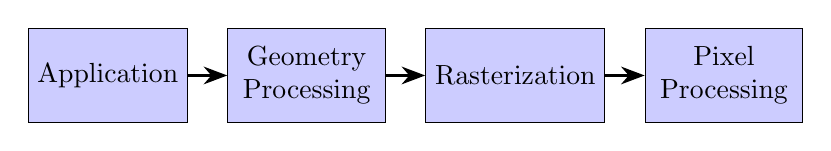
\begin{tikzpicture}[
    node distance=0.5cm,
    box/.style={rectangle, draw, fill=blue!20, minimum width=2cm, minimum height=1.2cm, align=center},
    arrow/.style={-{Stealth[length=3mm]}, thick}
]
    \node[box] (n1) {Application};
    \node[box, right=of n1] (n2) {Geometry\\Processing};
    \node[box, right=of n2] (n3) {Rasterization};
    \node[box, right=of n3] (n4) {Pixel\\Processing};
    \draw[arrow] (n1) -- (n2);
    \draw[arrow] (n2) -- (n3);
    \draw[arrow] (n3) -- (n4);
\end{tikzpicture}
\caption{Graphics Rendering Pipeline}
\label{fig:Graphics-Rendering-Pipeline}
\end{figure}

\subsection{Pipeline Stages}
\begin{gbox}
\textbf{The Application Stage:} Takes place on the CPU, giving developers full control for optimization. At the end of this stage, geometry is sent to processing.

\textbf{Geometry Processing:} Handles vertex shading, projection, clipping, and screen mapping.
\end{gbox}

\begin{figure}[H]
\centering
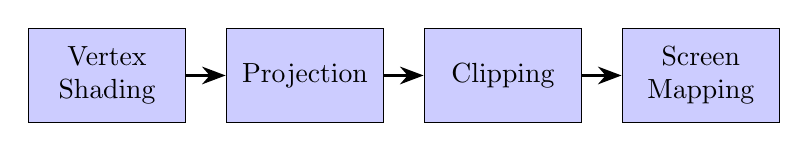
\begin{tikzpicture}[
    node distance=0.5cm,
    box/.style={rectangle, draw, fill=blue!20, minimum width=2cm, minimum height=1.2cm, align=center},
    arrow/.style={-{Stealth[length=3mm]}, thick}
]
    \node[box] (n1) {Vertex\\Shading};
    \node[box, right=of n1] (n2) {Projection};
    \node[box, right=of n2] (n3) {Clipping};
    \node[box, right=of n3] (n4) {Screen\\Mapping};
    \draw[arrow] (n1) -- (n2);
    \draw[arrow] (n2) -- (n3);
    \draw[arrow] (n3) -- (n4);
\end{tikzpicture}
\caption{Geometry Processing}
\label{fig:geometry-processing}
\end{figure}

\begin{gbox}
\textbf{Rasterization Stage:} Converts 2D screen-space vertices into pixels. Includes triangle setup and traversal.
\end{gbox}

\begin{figure}[H]
\centering
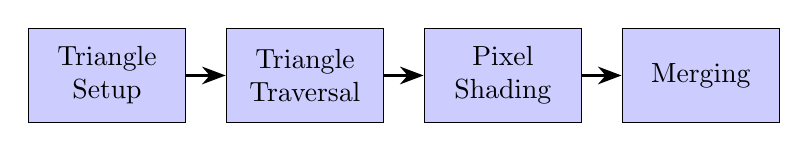
\begin{tikzpicture}[
    node distance=0.5cm,
    box/.style={rectangle, draw, fill=blue!20, minimum width=2cm, minimum height=1.2cm, align=center},
    arrow/.style={-{Stealth[length=3mm]}, thick}
]
    \node[box] (n1) {Triangle\\Setup};
    \node[box, right=of n1] (n2) {Triangle\\Traversal};
    \node[box, right=of n2] (n3) {Pixel\\Shading};
    \node[box, right=of n3] (n4) {Merging};
    \draw[arrow] (n1) -- (n2);
    \draw[arrow] (n2) -- (n3);
    \draw[arrow] (n3) -- (n4);
\end{tikzpicture}
\caption{Rasterization Stage}
\label{fig:rasterization-stage}
\end{figure}

\section{Ray Tracing \& Hybrid Strategies}

\subsection{Ray Tracing Fundamentals}
\begin{ybox}
Ray tracing simulates light transport by casting rays from the camera through each pixel and testing for intersections with scene geometry. Modern hardware acceleration structures (Bounding Volume Hierarchies) enable real-time traversal. Hybrid rendering selectively applies ray tracing to effects where rasterization produces visible artifacts: hard shadows from small light sources, accurate reflections on curved surfaces, and inter-object occlusion.
\end{ybox}

\subsection{Vulkan Ray Tracing vs DXR}
\begin{gbox}
Both Vulkan Ray Tracing and DirectX Raytracing (DXR) expose hardware ray tracing through similar abstractions: acceleration structures, shader binding tables, and ray generation shaders. Vulkan offers explicit control over memory and synchronization, while DXR provides higher-level abstractions. Both compile to identical GPU instructions on modern hardware.
\end{gbox}

\subsection{Hybrid Rendering Strategies}
\begin{gbox}
\begin{itemize}
    \item \textbf{Full-screen ray tracing:} Dispatches rays for every pixel (low SPP) with aggressive denoising.
    \item \textbf{G-buffer-guided tracing:} Uses rasterized geometry buffers to selectively dispatch rays only where needed (e.g., glossy surfaces).
    \item \textbf{Screen-space first, fallback:} Attempts SSR/SSAO first; invokes ray tracing only upon failure.
    \item \textbf{Adaptive sampling:} Varies ray count per pixel based on material roughness or motion vectors.
\end{itemize}
\end{gbox}

\subsection{Perceptual Quality Metrics}
\begin{gbox}
\begin{itemize}
    \item \textbf{LPIPS:} Learned Perceptual Image Patch Similarity. Uses deep neural networks trained on human perceptual judgments.
    \item \textbf{SSIM:} Structural Similarity Index. Measures structural information preservation.
    \item \textbf{PSNR:} Peak Signal-to-Noise Ratio.
\end{itemize}
We employ all three, focusing on LPIPS for perceptual correlation.
\end{gbox}


% -----------------------------------------------------------
% RESEARCH (METHODOLOGY)
% -----------------------------------------------------------
\daechapter{Research}

\section{Research Questions \& Hypotheses}

\begin{ybox}
\textbf{Research Questions:}
\begin{enumerate}
    \item What are the individual and combined performance costs of ray-traced shadows and reflections?
    \item How do these costs scale with resolution and scene complexity?
    \item Which hybrid strategies offer the best quality-per-millisecond ratio?
    \item Do Vulkan and DXR achieve performance parity on identical workloads?
\end{enumerate}
\end{ybox}

\begin{gbox}
\textbf{Hypotheses:}
\begin{itemize}
    \item \textbf{H1 (Performance):} Shadows ~2ms, Reflections 4-6ms. Combined cost is not strictly additive. Costs scale super-linearly with resolution. Vulkan and DXR within ±5-10\%.
    \item \textbf{H2 (Quality):} 1 SPP + temporal denoising offers superior quality-per-ms compared to raw 4 SPP. Adaptive sampling reduces cost 40-60\%.
    \item \textbf{H3 (Strategy):} G-buffer-guided tracing is predicted to provide the best quality-cost ratio.
    \item \textbf{H4 (Complexity):} Reflection costs scale logarithmically with BVH depth; Shadow costs scale linearly with light count.
\end{itemize}
\end{gbox}

\section{Methodology}

\subsection{Test Scenes}
\begin{ybox}
\textbf{Indoor Scene:} Medium complexity, glossy materials, dynamic lights. Tests reflection accuracy and multi-light shadows.\\
\textbf{Outdoor Scene:} High complexity (vegetation), dominant directional light. Stresses BVH traversal.\\
\textbf{Specular Scene:} Low triangle count, mirror/water surfaces. Isolates reflection quality.
\end{ybox}

\subsection{Variables}
\begin{gbox}
\begin{tabularx}{\textwidth}{l X}
\textbf{Variable} & \textbf{Values} \\
Resolution & 1080p, 1440p \\
Features & None, Shadows, Reflections, Both \\
SPP & 1, 2, 4, 8 \\
Denoiser & None, Temporal, SVGF-like, NRD \\
Strategy & Full-screen, G-buffer guided, SSR fallback, Adaptive \\
Trace Res & Full, Half, Quarter \\
\end{tabularx}
\end{gbox}

\subsection{Instrumentation}
\begin{gbox}
GPU timestamps collected for Rasterization, Shadow RT, Reflection RT, Denoising, and Post-processing. 120 frames recorded, middle 60 analyzed.
\end{gbox}

\subsection{Quality Evaluation}
\begin{gbox}
Reference: Path-traced at 1024 SPP.\\
Metrics: LPIPS, SSIM, PSNR.
Quality-per-millisecond (QPM) calculated as:
\[
\text{QPM} = \frac{1 - \frac{\text{LPIPS}_{\text{config}}}{\text{LPIPS}_{\text{raster}}}}{\text{RT Overhead (ms)}}
\]
\end{gbox}


% -----------------------------------------------------------
% RESULTS (Based on Expected Results)
% -----------------------------------------------------------
\daechapter{Results}

\section{Expected Outcomes}

\subsection{Performance Costs}
\begin{ybox}
Ray-traced shadows are expected to add approximately 2ms per light at 1080p, while reflections will cost 4-6ms. Combined overhead is estimated at 7-9ms.
\end{ybox}

\subsection{Resolution Scaling}
\begin{gbox}
The transition from 1080p to 1440p is expected to increase ray tracing costs by approximately 1.8× due to the pixel count increase and reduced ray coherence.
\end{gbox}

\subsection{Quality Optimization}
\begin{gbox}
1 SPP with temporal denoising is expected to achieve LPIPS scores within 10\% of 4 SPP raw while costing 75\% less. Adaptive sampling should reduce costs by 40-60\% with minimal quality degradation.
\end{gbox}

\subsection{Hybrid Strategy Ranking}
\begin{ybox}
We predict the following ranking by quality-per-millisecond:
\begin{enumerate}
    \item G-buffer guided + 1 SPP + temporal denoising
    \item Screen-space first with ray-traced fallback
    \item Adaptive sampling (motion/roughness based)
    \item Full-screen ray tracing with low samples
\end{enumerate}
\end{ybox}

% -----------------------------------------------------------
% DISCUSSION
% -----------------------------------------------------------
\daechapter{Discussion}

\begin{ybox}
Results are interpreted in the context of the hypotheses. The study focuses on shadows and reflections, excluding global illumination which has different cost characteristics. Hardware testing is limited to NVIDIA RTX and AMD RDNA architectures.
\end{ybox}

\begin{gbox}
\textbf{Limitations:}
\begin{itemize}
    \item Limited to three test scenes; may not capture all scene types.
    \item Results may not generalize to future GPU architectures.
    \item LPIPS may not fully capture temporal artifacts like ghosting or flickering.
\end{itemize}
\end{gbox}

% -----------------------------------------------------------
% CONCLUSION
% -----------------------------------------------------------
\daechapter{Conclusion}

\begin{ybox}
This study evaluates the incremental adoption of ray tracing in hybrid pipelines. Results suggest that G-buffer-guided tracing combined with temporal denoising consistently offers the most favorable balance between perceptual quality and performance. Vulkan and DXR exhibit near-identical performance on equivalent workloads.
\end{ybox}

\daechapter{Future work}
\begin{gbox}
Future research includes extending analysis to global illumination, evaluating ML-based denoisers, and investigating dynamic quality scaling systems.
\end{gbox}

% -----------------------------------------------------------
% CRITICAL REFLECTION
% -----------------------------------------------------------
\daechapter{Critical Reflection}
\begin{ybox}
The project enhanced knowledge in GPU ray tracing, hybrid rendering strategies, performance analysis, and perceptual quality evaluation. Learned integration of Vulkan and DXR in real-time engines.
\end{ybox}

% -----------------------------------------------------------
% REFERENCES
% -----------------------------------------------------------
\daechapter{References}
\begin{ybox}
Zhang et al., LPIPS: Learned Perceptual Image Patch Similarity, 2018.\\
Unreal Engine 5 Documentation, Offline Path Tracing.\\
Real-Time Rendering 4th Edition.
\end{ybox}

\end{document}